% VeriReason research idea proposal (Beamer). Rebuilt on 15 Oct 2026 from the 5 Oct 2026 PDF,
% with the corrections in docs/SLIDE_CORRECTIONS.md and the dates of the Project Timeline.
% Build: cd slides && pdflatex VeriReason_Proposed_Slide.tex (twice)
\documentclass[aspectratio=169,10pt]{beamer}
\usepackage[T1]{fontenc}
\usepackage{lmodern}
\usepackage{amsmath,amssymb}
\usepackage[table]{xcolor}
\usepackage{booktabs,array,tabularx,multirow,colortbl}
\usepackage{graphicx}
\usepackage{pifont}
\usepackage{tikz}
\usetikzlibrary{arrows.meta,positioning,shadows}

\newcolumntype{L}[1]{>{\raggedright\arraybackslash}p{#1}}
\newcolumntype{Y}{>{\raggedright\arraybackslash}X}
\definecolor{vrblue}{RGB}{31,78,121}
\definecolor{vrdark}{RGB}{28,63,102}
\definecolor{vrlight}{RGB}{232,238,245}
\definecolor{vrred}{RGB}{253,228,228}
\definecolor{vrgreen}{RGB}{226,242,229}

\newcommand{\vrdate}{15 October 2026}

% ---------- theme ----------
\usetheme{default}
\setbeamercolor{structure}{fg=vrblue}
\setbeamercolor{normal text}{fg=black}
\setbeamerfont{block title}{series=\bfseries,size=\normalsize}
\setbeamercolor{block title}{fg=white,bg=vrdark}
\setbeamercolor{block body}{fg=black,bg=vrlight}
\setbeamertemplate{navigation symbols}{}
\setbeamertemplate{itemize item}{\raisebox{0.1ex}{\scalebox{0.7}{$\bullet$}}}
\setbeamertemplate{itemize subitem}{\raisebox{0.1ex}{\scalebox{0.55}{$\bullet$}}}
\setbeamertemplate{enumerate item}{\tikz[baseline=(n.base)]\node[circle,fill=vrblue,text=white,inner sep=1.2pt,font=\scriptsize\bfseries](n){\insertenumlabel};}
\setbeamercolor{item}{fg=vrblue}
\setbeamertemplate{background}{
\includegraphics[width=\paperwidth,height=\paperheight]{img/bg_content.jpg}}
\setbeamercolor{frametitle}{fg=white,bg=vrblue}
\setbeamerfont{frametitle}{series=\bfseries,size=\Large}
\setbeamertemplate{footline}{%
  \leavevmode
  \begin{tikzpicture}[remember picture,overlay]
    \node[anchor=south east,xshift=-2mm,yshift=5mm,inner sep=0] at (current page.south east)
      {
\includegraphics[height=0.62cm]{img/f_uts.png}\hspace{3pt}
\includegraphics[height=0.62cm]{img/f_bk.png}};
  \end{tikzpicture}%
  \hbox{%
    \begin{beamercolorbox}[wd=.34\paperwidth,ht=2.4ex,dp=1ex,leftskip=1ex]{footer}%
      \usebeamerfont{footnote}\color{white}Nguyen Minh Quan, Tran Hai My\end{beamercolorbox}%
    \begin{beamercolorbox}[wd=.33\paperwidth,ht=2.4ex,dp=1ex,center]{footer}%
      \usebeamerfont{footnote}\color{white}VeriReason\end{beamercolorbox}%
    \begin{beamercolorbox}[wd=.33\paperwidth,ht=2.4ex,dp=1ex,rightskip=1ex,right]{footer}%
      \usebeamerfont{footnote}\color{white}Idea Proposal\quad\insertframenumber\,/\,\inserttotalframenumber\end{beamercolorbox}}}
\setbeamercolor{footer}{bg=vrdark}
\setbeamerfont{footnote}{size=\scriptsize}

% frame title bar
\setbeamersize{text margin left=2.2em,text margin right=2.2em}
\addtobeamertemplate{frametitle}{}{\vspace*{0.35cm}}
\setbeamertemplate{frametitle}{%
  \begin{tikzpicture}[remember picture,overlay]
    \node[anchor=north west,inner sep=0,fill=vrblue,text=white,minimum width=.975\paperwidth,minimum height=0.95cm,
          text width=.95\paperwidth,align=left,font=\Large\bfseries] at (current page.north west)
      {\hspace*{0.2cm}\insertframetitle};
  \end{tikzpicture}%
  \vskip1.2ex}
\setbeamertemplate{headline}{}

% section divider
\newcommand{\sectionslide}[2]{%
  {\setbeamertemplate{background}{
\includegraphics[width=\paperwidth,height=\paperheight]{img/bg_content.jpg}}%
   \setbeamertemplate{footline}{}\setbeamertemplate{headline}{}%
   \begin{frame}[plain]
     \begin{tikzpicture}[remember picture,overlay]
       \node[anchor=north west,xshift=4mm,yshift=-3mm,inner sep=0] at (current page.north west)
         {
\includegraphics[height=0.7cm]{img/f_uts.png}\hspace{4pt}
\includegraphics[height=0.7cm]{img/f_bk.png}};
       \node[anchor=center,yshift=14mm] at (current page.center) {\small Section #1};
       \node[anchor=center,fill=vrdark,text=white,rounded corners=4pt,minimum width=.96\paperwidth,minimum height=1.1cm,
             font=\Large\bfseries,yshift=-2mm] at (current page.center) {#2};
     \end{tikzpicture}
   \end{frame}}}

\newcommand{\tick}{\textcolor{green!45!black}{\ding{51}}}
\newcommand{\cross}{\textcolor{red!70!black}{\ding{55}}}
\setlength{\leftmargini}{1.4em}

\title{VeriReason}
\author{Nguyen Minh Quan, Tran Hai My}
\date{\vrdate}

\begin{document}

% ---------------- 1 title ----------------
{\setbeamertemplate{background}{
\includegraphics[width=\paperwidth,height=\paperheight]{img/bg_title.jpg}}%
\setbeamertemplate{footline}{}\setbeamertemplate{headline}{}%
\begin{frame}[plain]
  \begin{tikzpicture}[remember picture,overlay]
    \node[anchor=north,yshift=-2mm,inner sep=0] at (current page.north)
      {
\includegraphics[height=0.85cm]{img/t_vnu.png}\hspace{10pt}
\includegraphics[height=0.85cm]{img/t_bk.png}\hspace{10pt}
\includegraphics[height=0.85cm]{img/t_uts.png}\hspace{10pt}
\includegraphics[height=0.85cm]{img/t_ura.png}};
    \node[anchor=south,yshift=2mm,inner sep=0] at (current page.south)
      {
\includegraphics[width=.55\paperwidth]{img/t_bottom.png}};
    \node[anchor=center,align=center,yshift=2mm,text width=.9\paperwidth] at (current page.center) {%
      {\Large\bfseries\color{vrblue} VeriReason:\\ Intervention-Based Claim Verification and Repair\\ for LLM-Generated Credit Denial Explanations}\\[3.2ex]
      {\normalsize Supervisor: Assoc.\ Prof.\ Quan Thanh Tho\\ Students: Nguyen Minh Quan, Tran Hai My}\\[2.2ex]
      {\footnotesize Faculty of Computer Science and Engineering\\ Ho Chi Minh City University of Technology\\ Vietnam National University Ho Chi Minh City\\ University of Technology Sydney}\\[2.2ex]
      {\normalsize Research Idea Proposal\\ \vrdate\ (updated; first presented 5 October 2026)}};
  \end{tikzpicture}
\end{frame}}

% ---------------- 2 TOC ----------------
\begin{frame}{Table of Contents}
  \vspace{1ex}
  \begin{enumerate}
    \setlength{\itemsep}{1.2ex}
    \item Motivation
    \item Problem Statement
    \item Related Work
    \item Proposed Method
    \item Experimental Plan
    \item Expected Contributions
  \end{enumerate}
\end{frame}

% ---------------- 3 ----------------
\sectionslide{1}{Motivation}

% ---------------- 4 ----------------
\begin{frame}{Why Claim-Level Verification?}
  \vspace{2ex}
  \begin{itemize}
    \setlength{\itemsep}{1.1ex}
    \item[\textbullet] {\color{vrblue}\bfseries Requirement.} A denial must state the \emph{specific, principal reasons} (Regulation B, 12 CFR 1002.9 and its Official Interpretation).
    \item[\textbullet] {\color{vrblue}\bfseries Practice.} Reasons come from SHAP and are now rewritten into plain language by LLMs.
    \item[\textbullet] {\color{vrblue}\bfseries Problem.} Studies report that LLMs name the influential factors but are less reliable on \emph{direction}; a fluent, wrong reason is a compliance risk.
    \item[\textbullet] {\color{vrblue}\bfseries Gap.} Evaluations score the whole text, not which sentence is wrong or how to fix it.
    \item[\textbullet] {\color{vrblue}\bfseries Need.} Check every claim against the model; repair only the claims that fail.
  \end{itemize}
  \vfill{\footnotesize Regulation B and its Official Interpretation remain in force; CFPB Circular 2022-03 was withdrawn on 12 May 2025 and is background only.}\vspace{4ex}
\end{frame}

% ---------------- 5 ----------------
\begin{frame}{Objectives and Scope}
  \begin{block}{Goal}
    A verification-and-repair framework that checks each claim of an LLM-generated credit denial explanation against the behavior of the scoring model, identifies the type of each error, and selectively repairs only the claims that fail.
  \end{block}
  \vspace{1ex}
  \begin{columns}[T]
    \begin{column}{.48\textwidth}
      {\small\bfseries Objectives}
      \begin{enumerate}\small
        \setlength{\itemsep}{0.8ex}
        \item Define an error taxonomy grounded in the principal-reasons requirement.
        \item Decompose LLM explanations into typed, checkable claims.
        \item Verify each claim against the scoring model through dependency-aware interventions.
        \item Repair only the claims that fail, preserving supported content.
      \end{enumerate}
    \end{column}
    \begin{column}{.48\textwidth}
      {\small\bfseries Scope}
      \begin{itemize}\small
        \setlength{\itemsep}{0.8ex}
        \item Tabular credit scoring: gradient-boosted trees (primary), logistic regression (validation)
        \item English explanations for denied applicants, from several LLMs and prompting setups
        \item Public credit datasets; TreeSHAP attributions
        \item Not covered: legal-compliance certification, fairness auditing, multimodal models, explanation drift
      \end{itemize}
    \end{column}
  \end{columns}
\end{frame}

% ---------------- 6 ----------------
\begin{frame}{Research Questions}
  \begin{block}{RQ1\quad Error Characterization}
    How often, and in which ways (factor, direction, magnitude, omission, specificity), do LLM-generated credit denial explanations contradict the behavior of the scoring model?
  \end{block}
  \begin{block}{RQ2\quad Verification}
    Does dependency-aware, intervention-based verification detect these errors more reliably than attribution-sign checks, LLM judges, and general claim-verification frameworks?
  \end{block}
  \begin{block}{RQ3\quad Repair}
    Can selective claim-level repair reduce errors while preserving supported claims, compared with full regeneration and claim filtering?
  \end{block}
\end{frame}

% ---------------- 7 ----------------
\sectionslide{2}{Problem Statement}

% ---------------- 8 ----------------
\begin{frame}{Setting and Notation}
  \vspace{1.5ex}
  \begin{itemize}
    \setlength{\itemsep}{1.2ex}
    \item[\textbullet] Scoring model $f:\mathcal{X}\to[0,1]$ (predicted default risk); applicant $x$ is denied when $f(x)\ge\tau$.
    \item[\textbullet] Features are partitioned into {\color{vrblue}\bfseries reason groups} $G=\{g_1,\dots,g_K\}$: payment history, credit utilization, recent inquiries, income and affordability.
    \item[\textbullet] $\varphi(x)$ is the TreeSHAP attribution of $f$ at $x$. An LLM writes an explanation $e$ from $(x,f(x),\varphi(x))$; some setups omit $\varphi(x)$.
    \item[\textbullet] An extractor splits $e$ into claims $C=\{c_1,\dots,c_m\}$, each $c_j=(g_j,\delta_j,\mu_j)$ with its text span:
    \begin{itemize}
      \item $\delta_j\in\{\text{raises risk},\text{lowers risk},\text{neutral}\}$\quad (stated direction)
      \item $\mu_j\in\{\text{principal},\text{contributing},\text{minor}\}$\quad (stated prominence)
    \end{itemize}
  \end{itemize}
\end{frame}

% ---------------- 9 ----------------
\begin{frame}{Reference Effect}
  \[\Delta_g(x)=f(x)-\mathbb{E}_{\tilde x_g\sim Q_g(\cdot\mid x_{-g})}\Bigl[f\bigl(h(\tilde x_g,x_{-g})\bigr)\Bigr]\]
  \begin{itemize}\footnotesize
    \setlength{\itemsep}{0.9ex}
    \item[\textbullet] $x_{-g}$: the applicant's features outside $g$; $\tilde x_g$: a plausible alternative value of group $g$.
    \item[\textbullet] $Q_g$: conditional (on-manifold) sampler on a reference population; $h$ recomputes derived features (e.g., debt-to-income).
    \item[\textbullet] Verified direction $\widehat{\delta}_g=\operatorname{sign}_\varepsilon\bigl(\Delta_g(x)\bigr)\in\{+,0,-\}$: $\Delta_g(x)>\varepsilon$ means the applicant's values in $g$ \emph{raise} predicted risk.
    \item[\textbullet] Risk-increasing groups $G^+=\{g:\Delta_g(x)>\varepsilon\}$, ranked by $\Delta_g(x)$; principal reasons are the top $k$ of $G^+$ (Reg.\ B commentary: usually $k\le 4$).
  \end{itemize}
  \vspace{0.5ex}
  \begin{block}{A defined reference, not ground truth}
    $\Delta_g(x)$ depends on $Q_g$ and the reference population: verdicts are reported under several references.
  \end{block}
\end{frame}

% ---------------- 10 ----------------
\begin{frame}{Error Taxonomy}
  \vspace{0.5ex}
  \scriptsize
  \renewcommand{\arraystretch}{1.25}
  \begin{tabularx}{\textwidth}{@{}l L{1.5cm} L{3.0cm} L{3.3cm} Y@{}}
    \textbf{\color{vrblue}ID} & \textbf{\color{vrblue}Error} & \textbf{\color{vrblue}Meaning} & \textbf{\color{vrblue}Example} & \textbf{\color{vrblue}Check}\\\hline
    E1 & Unsupported factor & Described as contributing, but no meaningful effect, or not a model input & ``Your age counted against you'' (age not used) & $\delta_j\ne\text{neutral}$ but $\widehat\delta_g=0$, or $g$ not an input\\
    E2 & Wrong direction & Stated direction opposite to model behavior & ``No prior loans raised your risk'' (model: neutral or favorable) & $\widehat\delta_g\ne0$ and $\widehat\delta_g\ne\delta_j$\\
    E3 & Wrong prominence & Minor factor shown as principal, or the reverse & Small inquiry effect listed as the main reason & rank of $g$ in $G^+$ vs.\ $\mu_j$\\
    E4 & Omission & A verified principal group is missing & Top driver (utilization) never mentioned & $\mathrm{Top}_k(G^+)$ vs.\ mentioned groups\\
    E5 & Non-specific & Cannot be mapped to a group, or too generic & ``Your overall credit profile was weak'' & flagged non-checkable\\
    E6 & Invalid recourse (optional) & Action would not change the decision, or targets an immutable attribute & ``Increase your income by 2\%'' (no flip) & $f(h(x'))\ge\tau$ for the suggested $x'$, or immutable $g$
  \end{tabularx}
  \vspace{1ex}

  {\tiny $x'$: applicant profile after the suggested action. Ranking within $G^+$ uses the signed $\Delta_g(x)$, so a favorable group is never a reason for denial.}
\end{frame}

% ---------------- 11 ----------------
\sectionslide{3}{Related Work}

% ---------------- 12 ----------------
\begin{frame}{LLM Explanations in Credit and Finance}
  \vspace{1ex}
  \begin{itemize}\footnotesize
    \setlength{\itemsep}{1ex}
    \item[\textbullet] {\color{vrblue}\bfseries Zandi et al.\ (2026):} on Freddie Mac data, LLM narratives name influential factors reliably but are less reliable on direction.
    \item[\textbullet] {\color{vrblue}\bfseries Geng et al.\ (2026):} LLMs work best as narrative interfaces, not substitutes for formal attribution methods.
    \item[\textbullet] {\color{vrblue}\bfseries AlMarri et al.\ (2025):} when an LLM explains its own default predictions, its feature-impact statements often disagree with SHAP on financial tabular tasks (the LLM is the classifier there, unlike our setting).
    \item[\textbullet] {\color{vrblue}\bfseries LEXMA (2026):} RL fine-tuning for mortgage decisions; experts and consumers preferred it to the base model.
    \item[\textbullet] {\color{vrblue}\bfseries Principal reasons:} deployers take top attribution features; one lender groups SHAP values and adds a directionality score.
  \end{itemize}
  \vfill
  \begin{block}{Takeaway}
    LLM credit explanations can be wrong, yet none are verified by intervention or repaired claim by claim.
  \end{block}
  \vspace{4ex}
\end{frame}

% ---------------- 13 ----------------
\begin{frame}{Faithfulness and Claim Verification}
  \vspace{1ex}
  \begin{itemize}\footnotesize
    \setlength{\itemsep}{1ex}
    \item[\textbullet] {\color{vrblue}\bfseries FActScore, RARR:} atomic-fact scoring and evidence-grounded revision; not faithfulness to a model's behavior.
    \item[\textbullet] {\color{vrblue}\bfseries Counterfactual tests:} Atanasova et al.\ (2023), Siegel et al.\ (75 models, 13 families), Walk the Talk (2025); Faithful Serum (2026) adds attribution-guided steering.
    \item[\textbullet] {\color{vrblue}\bfseries FAX (2026):} decomposes drafts into claims and tests them with tools that query the target model; refuted claims are removed or rewritten, inconclusive ones are not presented as verified. Evaluated mainly outside credit (main benchmark: an RL environment); German Credit is one of three TalkToModel tabular sets, and the authors caution that such benchmarks can conflate task accuracy with model-specific faithfulness. \emph{Closest prior work.}
    \item[\textbullet] {\color{vrblue}\bfseries EDCT} (vision-language models), {\color{vrblue}\bfseries TalkToModel} (conversational tabular explanation).
  \end{itemize}
  \vfill
  \begin{block}{Takeaway}
    FAX is a main baseline. It has no notion of principal reasons, omission or prominence, and no constraint to preserve supported claims. Missing: a credit-specific taxonomy, interventions for correlated features, and repair that preserves supported claims; the pilot tests whether FAX suffices.
  \end{block}
  \vspace{3ex}
\end{frame}

% ---------------- 14 ----------------
\begin{frame}{Positioning}
  \vspace{0.5ex}
  \small
  \renewcommand{\arraystretch}{1.15}
  \begin{tabular}{@{}>{\columncolor{vrlight}}L{3.9cm} L{2.0cm} L{2.9cm} L{3.3cm} L{1.0cm}@{}}
    \textbf{\color{vrblue}Capability} & \textbf{\color{vrblue}LLM-in-credit} & \textbf{\color{vrblue}General faithfulness (CT/CCT, Serum)} & \textbf{\color{vrblue}FAX} & \textbf{\color{vrblue}Ours}\\\hline
    Credit-specific setting & Yes & No & Partial (German Credit only; mainly non-credit) & \textcolor{vrblue}{Yes}\\
    Claim-level decomposition & n/r & Partial & Yes & \textcolor{vrblue}{Yes}\\
    Intervention-based verification & n/r & Yes & Yes (faithful tools) & \textcolor{vrblue}{Yes}\\
    Credit error taxonomy & Partial (direction) & n/r & n/r & \textcolor{vrblue}{Yes}\\
    Correlated-feature interventions & n/r & n/r & n/r & \textcolor{vrblue}{Yes}\\
    Selective repair & n/r & Partial (steering) & Partial (remove or rewrite; no preservation constraint) & \textcolor{vrblue}{Yes}
  \end{tabular}
  \vspace{1ex}

  {\scriptsize n/r = not reported in an abstract-level reading, not proven absent; to be verified in full texts (Week 0).}
\end{frame}

% ---------------- 15 ----------------
\sectionslide{4}{Proposed Method}

% ---------------- 16 ----------------
\begin{frame}{Method Overview and Claim Extraction}
  \begin{block}{Core Question}
    Which claims contradict the model's behavior, what kind of error is each, and how can the explanation be repaired without changing supported claims?
  \end{block}
  \vspace{1.2ex}
  \begin{center}
  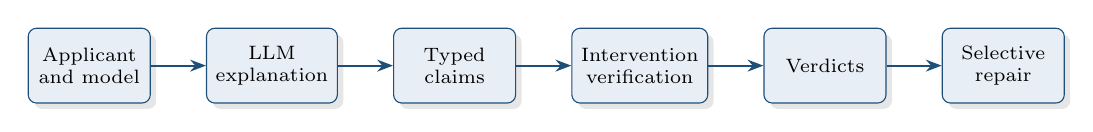
\begin{tikzpicture}[node distance=7mm,every node/.style={draw=vrblue,rounded corners=3pt,fill=vrlight,align=center,font=\scriptsize,minimum width=1.55cm,minimum height=0.95cm,drop shadow={opacity=0.2}},>={Stealth[length=2mm]}]
    \node (a) {Applicant\\and model};
    \node[right=of a] (b) {LLM\\explanation};
    \node[right=of b] (c) {Typed\\claims};
    \node[right=of c] (d) {Intervention\\verification};
    \node[right=of d] (e) {Verdicts};
    \node[right=of e] (f) {Selective\\repair};
    \foreach \x/\y in {a/b,b/c,c/d,d/e,e/f}{\draw[->,vrblue,thick] (\x) -- (\y);}
  \end{tikzpicture}
  \end{center}
  \begin{itemize}\small
    \setlength{\itemsep}{0.8ex}
    \item[\textbullet] An LLM extractor with a fixed schema returns group, direction, prominence, optional action, and the character span.
    \item[\textbullet] Spans are preserved so repair is local; unmappable claims are labeled E5, not discarded.
    \item[\textbullet] Extractor quality is measured on a manually annotated subset and carried into the ablations.
  \end{itemize}
\end{frame}

% ---------------- 17 ----------------
\begin{frame}{Dependency-Aware Verification}
  \vspace{1.5ex}
  \begin{itemize}\small
    \setlength{\itemsep}{1.1ex}
    \item[\textbullet] {\color{vrblue}\bfseries Group-level replacement:} related features move together; derived features are recomputed by $h$.
    \item[\textbullet] {\color{vrblue}\bfseries Plausible alternatives:} $Q_g$ is a conditional sampler (nearest neighbors in $x_{-g}$, or a conditional generative model), not independent marginals that create impossible profiles.
    \item[\textbullet] {\color{vrblue}\bfseries Claim verdicts:} supported, or E1, E2, E3, E5 (E6 for recourse claims), using $\widehat\delta_g$, the rank of $g$ in $G^+$, and the flip test.
    \item[\textbullet] {\color{vrblue}\bfseries Response level:} omission (E4) and consistency of principal reasons across near-identical applicants.
    \item[\textbullet] {\color{vrblue}\bfseries Reference sensitivity:} conditional sampler, population median, approved-applicant reference; a SHAP-sign verifier runs on the same claims.
    \item[\textbullet] Each verdict is stored with its evidence ($\Delta_g(x)$, rank, samples): an {\color{vrblue}\bfseries audit record}.
  \end{itemize}
\end{frame}

% ---------------- 18 ----------------
\begin{frame}{Selective Repair}
  \begin{columns}[T]
    \begin{column}{.62\textwidth}
      \vspace{1.5ex}
      \begin{enumerate}\small
        \setlength{\itemsep}{1.4ex}
        \item Build a fact sheet per flagged claim (group, verified direction, rank).
        \item Regenerate only the offending span, or insert a sentence for an omission.
        \item Re-verify; after a few attempts fall back to a templated sentence.
        \item Text diff: supported claims must stay verbatim.
      \end{enumerate}
    \end{column}
    \begin{column}{.34\textwidth}
      \centering\small
      {\bfseries Before}\\[0.5ex]
      \tick\ Payment history\\
      \cross\ \colorbox{vrred}{Inquiries (E3)}\\
      \tick\ Utilization\\[0.5ex]
      $\Downarrow$\\[0.5ex]
      {\bfseries After}\\[0.5ex]
      \tick\ Payment history\\
      \tick\ \colorbox{vrgreen}{Inquiries}\\
      \tick\ Utilization
    \end{column}
  \end{columns}
  \vfill
  \begin{block}{Preservation Objective}
    Supported claims remain unchanged; the number of edited spans equals the number of verified errors.
  \end{block}
  \vspace{4ex}
\end{frame}

% ---------------- 19 ----------------
\begin{frame}{Validating the Verifier}
  \vspace{1.5ex}
  \begin{itemize}\small
    \setlength{\itemsep}{1.3ex}
    \item[\textbullet] {\color{vrblue}\bfseries Logistic regression} $f(x)=\sigma(w^\top x+b)$: the group effect in logit space, $w_g^\top\bigl(x_g-\mathbb{E}_R[x_g]\bigr)$, is analytic and gives the true direction and ranking. We measure how often the verifier agrees with it.
    \item[\textbullet] {\color{vrblue}\bfseries Semi-synthetic credit model:} planted rules give known reasons per applicant, testing the verifier under correlated features and interactions.
    \item[\textbullet] {\color{vrblue}\bfseries Expert annotation:} a small set of XGBoost explanations labeled by annotators with credit or finance background.
  \end{itemize}
  \vfill{\footnotesize Note: with a conditional sampler and the sigmoid, $\Delta_g(x)$ itself is not closed-form; it is estimated by sampling.}\vspace{4ex}
\end{frame}

% ---------------- 20 ----------------
\sectionslide{5}{Experimental Plan}

% ---------------- 21 ----------------
\begin{frame}{Datasets, Models and Generators}
  \footnotesize
  \renewcommand{\arraystretch}{1.2}
  \begin{tabularx}{\textwidth}{@{}L{3.1cm} L{2.5cm} Y@{}}
    \textbf{\color{vrblue}Dataset} & \textbf{\color{vrblue}Role} & \textbf{\color{vrblue}Note}\\\hline
    Home Credit Default Risk & Primary (pilot) & Linked tables; Kaggle account and acceptance of the competition rules required; do not publish raw data\\
    German Credit (UCI, id 144) & Comparability & CC BY 4.0; used by prior work and as one of FAX's three tabular sets; added in Weeks 3--5\\
    FICO HELOC & Comparability (optional) & Request access via the FICO form; special negative codes need handling\\
    Lending Club / Freddie Mac & Secondary replication & Lending Club copy on Kaggle is user-uploaded: check its licence, remove leaking columns; Freddie Mac needs registration and cannot be redistributed
  \end{tabularx}
  \vspace{1.2ex}
  \begin{itemize}\footnotesize
    \setlength{\itemsep}{0.8ex}
    \item[\textbullet] {\color{vrblue}\bfseries Models:} XGBoost (primary; random forest if time permits), logistic regression (validation), TreeSHAP.
    \item[\textbullet] {\color{vrblue}\bfseries Caveat:} by default, TreeSHAP for XGBoost attributes the log-odds margin; these values add up in logit space, not probability space, so turning them into probability-scale statements is itself a possible source of error.
    \item[\textbullet] {\color{vrblue}\bfseries Generators:} 3--4 LLMs (small and large open-weight, one proprietary) $\times$ 3 prompts (features; +SHAP; +SHAP and group dictionary), several samples per applicant.
  \end{itemize}
\end{frame}

% ---------------- 22 ----------------
\begin{frame}{Baselines}
  \vspace{0.5ex}
  \small
  \renewcommand{\arraystretch}{1.35}
  \begin{tabularx}{\textwidth}{@{}l L{4.7cm} Y@{}}
    \textbf{\color{vrblue}ID} & \textbf{\color{vrblue}Baseline} & \textbf{\color{vrblue}What it tests}\\\hline
    B0 & Direct LLM explanation & Raw error rates without any verification\\
    B1 & Deterministic reason-code template from SHAP groups & Industry style: near-zero error, limited readability\\
    B2 & SHAP-sign verifier & Whether attribution signs suffice to check claims\\
    B3 & LLM-as-judge (with / without model access) & Whether a judge LLM detects direction and prominence errors\\
    B4 & FAX-style verify-and-filter (re-implemented for credit) & Closest general framework; central to the go/no-go decision\\
    B5 & RARR-style revision & Generic evidence-grounded selective revision\\
    B6 & Full regeneration with verified facts & Repair without selectivity; measures preservation cost
  \end{tabularx}
\end{frame}

% ---------------- 23 ----------------
\begin{frame}{Evaluation and Ablations}
  \begin{columns}[T]
    \begin{column}{.49\textwidth}
      {\small\bfseries\color{vrblue}Errors and verification (RQ1, RQ2)}
      \begin{itemize}\footnotesize
        \setlength{\itemsep}{0.7ex}
        \item Claim-level error rate by type (E1--E6); share of explanations with $\ge 1$ error
        \item Precision, recall, F1 per type vs.\ the reference (analytic on LR; expert labels on an XGBoost subset)
        \item SHAP-sign vs.\ intervention disagreement, split by feature correlation
      \end{itemize}
    \end{column}
    \begin{column}{.49\textwidth}
      {\small\bfseries\color{vrblue}Repair and cost (RQ3)}
      \begin{itemize}\footnotesize
        \setlength{\itemsep}{0.7ex}
        \item Residual error; supported claims unchanged; edit distance
        \item Principal-reason precision / recall vs.\ verified top-$k$; omission; stability
        \item Readability (LLM judge plus small human check); queries, LLM calls, latency
      \end{itemize}
    \end{column}
  \end{columns}
  \vspace{1.5ex}
  \begin{block}{Ablations}
    Dependency-aware vs.\ marginal sampling; group vs.\ single-feature; intervention vs.\ SHAP-sign verdicts; selective vs.\ full repair, with and without re-verification; reference, $\varepsilon$, extractor errors.
  \end{block}
\end{frame}

% ---------------- 24 ----------------
\begin{frame}{Pilot and Go/No-Go Gate}
  \small
  Two-week pilot (19 Oct--1 Nov 2026) on about 200 denied Home Credit applicants with three LLMs, the verifier, and the FAX-style baseline (B4); go/no-go meeting proposed for Mon 2 Nov 2026. Thresholds are pre-registered and illustrative.
  \vspace{0.8ex}
  \begin{itemize}\small
    \setlength{\itemsep}{1ex}
    \item[\textbullet] {\color{vrblue}\bfseries G1, problem exists:} at least 10\% of explanations have a direction, prominence, or omission error (E2, E3, E4).
    \item[\textbullet] {\color{vrblue}\bfseries G2, gap exists:} the FAX-style baseline leaves at least 30\% of the verifier's errors undetected or unrepaired (threshold proposed by the team).
    \item[\textbullet] {\color{vrblue}\bfseries G3, verifier is sound:} direction verdicts match the analytic LR reference: close to 100\% with the marginal sampler (implementation check), at least 95\% with the conditional kNN sampler.
  \end{itemize}
  \vfill
  \begin{block}{If the gate fails}
    If general verification already handles the errors, or LLM explanations are rarely wrong, reconsider the direction rather than forcing it.
  \end{block}
  \vspace{4ex}
\end{frame}

% ---------------- 25 ----------------
\sectionslide{6}{Expected Contributions}

% ---------------- 26 ----------------
\begin{frame}{Expected Contributions}
  \begin{enumerate}\small
    \setlength{\itemsep}{0.9ex}
    \item A regulation-informed error taxonomy and benchmark for credit denial explanations, with claim-level labels from model interventions.
    \item A dependency-aware, intervention-based claim verifier, with analysis of where SHAP-sign checks disagree.
    \item A selective claim-level repair procedure, compared with FAX-style filtering, RARR-style revision, and full regeneration.
    \item An empirical study across LLMs, prompts, and datasets of which errors occur and which strategies catch them.
  \end{enumerate}
  \vfill
  \begin{block}{Current Status and Next Steps}
    Initial idea from a targeted literature search; scaffold code, German Credit run and a pilot pre-registration are in place (\vrdate). Next: full-text review of FAX and the LLM-credit studies (Week 0), the two-week pilot (19 Oct--1 Nov) and the go/no-go meeting on 2 Nov, then refine or reconsider the direction.
  \end{block}
  \vspace{4ex}
\end{frame}

% ---------------- 27 ----------------
\begin{frame}{Risks and Mitigations}
  \scriptsize
  \renewcommand{\arraystretch}{1.25}
  \begin{tabularx}{\textwidth}{@{}L{3.1cm} Y@{}}
    \textbf{\color{vrblue}Risk} & \textbf{\color{vrblue}Mitigation}\\\hline
    Overlap with FAX & Re-implement it as B4; build on credit error types, correlated-feature interventions, preservation-aware repair; test the gap in the pilot\\
    Reference validity & State the definition openly; report sensitivity; validate on LR, semi-synthetic data, expert labels\\
    Implausible interventions & Group-level changes, derived-feature recomputation, conditional sampling; ablate against marginals\\
    LLM variance and cost & Several samples per applicant, fixed decoding, at least two open-weight models; fewer samples and cached outputs if over budget\\
    Regulatory overreach & Call the taxonomy regulation-informed; make no legal-compliance claim\\
    Data access and licensing & Start with Home Credit and German Credit; confirm terms of other sources\\
    Delay in Weeks 3--5 & Simplify the schema, keep only the kNN sampler, postpone the generative sampler\\
    No expert annotators & Ask the supervisor in Week 0; fallback: finance students with a written guide\\
    Application paper at an NLP venue & Stress benchmark, taxonomy, analysis of strategies; target a finance-NLP workshop first
  \end{tabularx}
\end{frame}

% ---------------- 28 ----------------
\begin{frame}{Timeline}
  \scriptsize
  \renewcommand{\arraystretch}{1.3}
  \begin{tabularx}{\textwidth}{@{}L{1.1cm} L{2.9cm} Y L{3.0cm}@{}}
    \textbf{\color{vrblue}Weeks} & \textbf{\color{vrblue}Dates} & \textbf{\color{vrblue}Work} & \textbf{\color{vrblue}Output / decision}\\\hline
    0 & 10--18 Oct 2026 & Supervisor meeting, full-text reading, data and licences, environment & Related-work table, working environment\\
    1--2 & 19 Oct--1 Nov & Data, reason groups, generators, pilot with FAX-style baseline & Go/no-go meeting, Mon 2 Nov\\
    3--5 & 2--22 Nov & Extractor, taxonomy, verifier, LR and semi-synthetic validation & Validated verifier\\
    6--8 & 23 Nov--13 Dec & Selective repair, remaining baselines & End-to-end system\\
    9--11 & 14 Dec--3 Jan 2027 & Full experiments, ablations, expert annotation & Main results\\
    12--13 & 4--17 Jan 2027 & Writing, figures, full-text related-work check & Submission draft
  \end{tabularx}
  \vspace{1.5ex}
  \begin{itemize}\footnotesize
    \setlength{\itemsep}{0.6ex}
    \item[\textbullet] Target: a finance-NLP workshop (e.g., FinNLP); ACL 2027 via ARR as a stretch goal (dates to be confirmed in Week 0).
    \item[\textbullet] Weeks 9--11 overlap with Christmas and New Year: schedule long generation and intervention jobs then.
    \item[\textbullet] Fallback scope if there is no end-to-end run by Week 8: drop Lending Club, Freddie Mac, random forest and E6.
  \end{itemize}
\end{frame}

% ---------------- 29 ----------------
{
\begin{frame}[plain]
  \vfill\centering{\Large\bfseries\color{vrblue} Thank you for your attention!}\vfill
\end{frame}}

\end{document}
